\documentclass[tikz,border=10pt]{standalone}
\usepackage{tikz-3dplot}
\usepackage{amsmath, amssymb}
\usetikzlibrary{arrows.meta, positioning, calc, decorations.pathreplacing, 3d}
\usetikzlibrary{matrix, fit, backgrounds, shapes}
\usetikzlibrary{angles,quotes}

\usepackage[T1]{fontenc}
\usepackage[utf8]{inputenc}
\usepackage{newpxtext,newpxmath}
\usepackage{sectsty}

\begin{document}
%========================================================
% TikZ #1 (Step 1): choose adapted basis
%========================================================
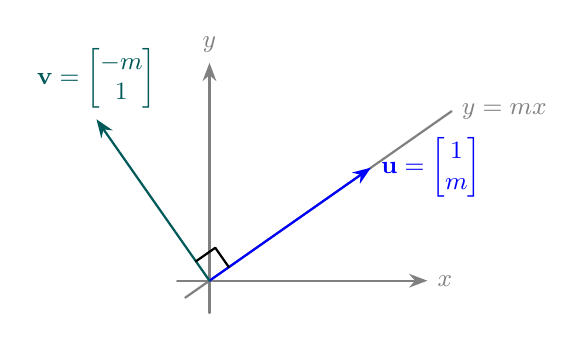
\begin{tikzpicture}[scale=2.05, >=Stealth, line cap=round, line join=round]
	\def\m{0.7}
	
	\pgfmathsetmacro{\ux}{1}
	\pgfmathsetmacro{\uy}{\m}
	\pgfmathsetmacro{\vxB}{-\m}
	\pgfmathsetmacro{\vyB}{1}
	
	\tikzset{
		axis/.style={thick, gray},
		axline/.style={thick, gray},
		uvec/.style={thick, blue},
		vvec/.style={thick, teal!70!black},
		box/.style={rounded corners, draw=gray!60, fill=white, inner sep=3pt},
		mat/.style={font=\small}
	}
	
	\newcommand{\panelaxes}{
		\draw[axis,->] (-0.2,0) -- (1.35,0) node[right] {\small $x$};
		\draw[axis,->] (0,-0.2) -- (0,1.35) node[above] {\small $y$};
	}
	
	\newcommand{\rightangleat}[3]{% X,Y,size
		\coordinate (RAU) at ({#1 + #3},{#2 + #3*\m});     % along axis
		\coordinate (RAN) at ({#1 - #3*\m},{#2 + #3});     % along normal
		\coordinate (RAC) at ({#1 + #3 - #3*\m},{#2 + #3*\m + #3});
		\draw[thick] (RAU) -- (RAC) -- (RAN);
	}
	
%	\node[box, anchor=west, align=center] at (-1.5,-0.5) {\small Step 1: Choose $\textbf{u}$ (along axis) and $\textbf{v}$ (perp)\\ ($\textbf{u}\cdot\textbf{v}=1\cdot(-m)+m\cdot 1=0$)};
	
	\panelaxes
	
	\draw[axline] (-0.15,{-0.15*\m}) -- (1.5,{1.5*\m})
	node[pos=1, right] {\small $y=mx$};
	
	\draw[uvec,->] (0,0) -- (\ux,\uy) node[pos=1, right] {\small $\textbf{u}=\begin{bmatrix}
			1 \\ m
		\end{bmatrix}$};
	\draw[vvec,->] (0,0) -- (\vxB,\vyB) node[pos=1, above] {\small $\textbf{v}=\begin{bmatrix}
			-m \\ 1
	\end{bmatrix}$};
	
	\rightangleat{0}{0}{0.12}
	
%	\node[anchor=west, mat] at (-0.18,1.05) {$u\cdot v=0$ so $\{u,v\}$ is a basis.};
	
\end{tikzpicture}
\end{document}